\documentclass[10pt]{beamer}

\input{/Users/danielschreurs/Documents/LaTeX/beamer-style.tex}

\title{Systèmes de Gestion de Bases de Données - 2\textsuperscript{e}}
\subtitle{PL-SQL - Chapitre 3 - Les structures de contrôle}
\date{\today}
\author{Daniel Schreurs}
\institute{Haute École de Province de Liège}
%\titlegraphic{\hfill\includegraphics[height=1.5cm]{logo.eps}}


\setbeamertemplate{frame footer}{\insertsectionhead}
\begin{document}
\maketitle

\setbeamerfont{subsection in toc}{size=\small}
\setbeamerfont{subsubsection in toc}{size=\normalsize}
\setbeamertemplate{section in toc}[sections numbered]
\setbeamertemplate{subsection in toc}[subsections numbered]
\setbeamertemplate{subsubsection in toc}[subsubsections numbered]
\begin{frame}[allowframebreaks]{Table des matières du chapitre}
    \tableofcontents[subsectionstyle=show/show/hide,subsubsectionstyle=show/show/hide,]
\end{frame}

\section{Introduction}
\tocss
\begin{frame}{\secname}
    \begin{figure}
        \begin{center}
            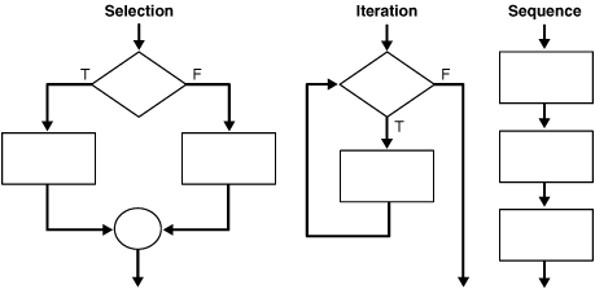
\includegraphics[width=0.8\textwidth]{../assets/img/structure-controle-rappel.png}
            \caption{Structure de contrôle rappel}
        \end{center}
    \end{figure}
\end{frame}

\section{Les structures conditionnelles}
\tocss
\subsection{IF THEN}
\begin{frame}{\secname : \subsecname}
    \begin{itemize}
        \item   Les instructions comprises dans la branche \lstinline[language=sql]!THEN! ne sont exécutées que si la condition est évaluée à \lstinline[language=sql]!true!.
        \item Si la condition est évaluée à \lstinline[language=sql]!false! ou \lstinline[language=sql]!UNKNOWN!, le contrôle passe à l'instruction qui suit le \lstinline[language=sql]!END IF!.
    \end{itemize}
\end{frame}

\begin{frame}{\secname : \subsecname}
    \lstinputlisting[language=sql, title=Une variable UNKNOWN]{../exemples/PLSQL Chapitre 3/if-then.sql}
\end{frame}

\begin{frame}{\secname : \subsecname}
    \lstinputlisting[language=sql, title=L'évaluation des conditions en PL/SQL suit le principe de l'évaluation rapide (short-circuit evaluation).
    ]{../exemples/PLSQL Chapitre 3/if-then-2.sql}
\end{frame}

\subsection{IF THEN ELSE}
\begin{frame}{\secname : \subsecname}
    \lstinputlisting[language=sql, title=Écriture douteuse]{../exemples/PLSQL Chapitre 3/IF-THEN-ELSE.sql}
\end{frame}

\begin{frame}{\secname : \subsecname}
    \lstinputlisting[language=sql, title=Test valide]{../exemples/PLSQL Chapitre 3/IF-THEN-ELSE-2.sql}
\end{frame}

\subsection{Case}
\begin{frame}{\secname : \subsecname}
    \lstinputlisting[language=sql, title=Structure CASE - valeur]{../exemples/PLSQL Chapitre 3/case.sql}
\end{frame}

\begin{frame}{\secname : \subsecname}
    \lstinputlisting[language=sql, title=Structure CASE - expression]{../exemples/PLSQL Chapitre 3/case2.sql}
\end{frame}

\section{Les structures itératives}
\tocss
\subsection{While}
\begin{frame}{\secname : \subsecname}
    \lstinputlisting[language=sql, title=Structure while]{../exemples/PLSQL Chapitre 3/while.sql}
\end{frame}

\subsection{For}
\begin{frame}{\secname : \subsecname}
    \begin{itemize}
        \item L'instruction \lstinline[language=sql]!FOR! permet de définir une boucle.
        \item Le nombre d'itérations est défini entre 2 entiers.
        \item La séquence d'instructions est exécutée pour chaque entier compris dans l'intervalle défini.
    \end{itemize}
    \metroset{block=fill}
    \begin{alertblock}{Important}
        Cet indice est défini implicitement dans la boucle !
    \end{alertblock}
\end{frame}

\begin{frame}{\secname : \subsecname}
    \lstinputlisting[language=sql, title=Structure for]{../exemples/PLSQL Chapitre 3/for.sql}
    \metroset{block=fill}
    \begin{alertblock}{Important}
        La variable Viteration n'est pas déclarée !!
    \end{alertblock}
\end{frame}

\begin{frame}{\secname : \subsecname}
    \lstinputlisting[language=sql, title=Erreur d'affectation]{../exemples/PLSQL Chapitre 3/for-2.sql}
\end{frame}

\begin{frame}{\secname : \subsecname}
    \lstinputlisting[language=sql, title=Portée]{../exemples/PLSQL Chapitre 3/for-3.sql}
\end{frame}

\begin{frame}{\secname : \subsecname}
    \begin{itemize}
        \item La variable \lstinline[language=sql]!Viteration! qui est explicitement déclarée est occultée dans la boucle par la variable compteur.
        \item On ne sait donc pas, dans la boucle, accéder à cette variable déclarée (sauf si on utilise un label)
        \item En dehors de la boucle, on ne peut accéder que à la variable Viteration déclarée, plus à la variable qui sert de compteur !!!
    \end{itemize}
\end{frame}

\end{document}